\twocolumn

\chapter{Система ограждения МАМС}\label{app:mams}

Система включает плавучие знаки пяти типов:
\begin{enumerate}
\item латеральные;
\item кардинальные;
\item ограждающие отдельные опасности;
\item обозначающие начальные точки и ось фарватера (канала) и середину прохода (осевые, или знаки чистой воды);
\item специального назначения.
\end{enumerate}

Мировой океан разделен на два региона (\rris{mams-map}): регион А и регион Б, которые
отличаются принципом использования красного и зелёного цветов для
ограждения сторон фарватера латеральными знаками.

\begin{figure*}[!htb]
  \centering{}
  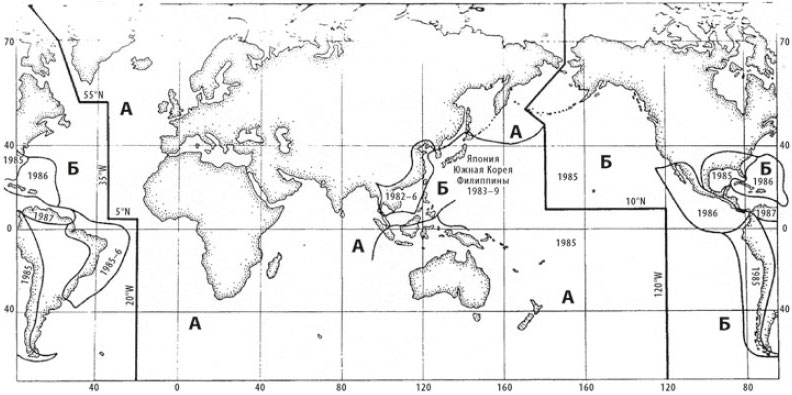
\includegraphics[width=\linewidth]{mams_map.jpeg}
  \caption{Деление на регионы}
  \label{fig:mams-map}
\end{figure*}

Страны, принявшие красный цвет окраски средств навигационного
оборудования (СНО) с левой стороны фарватера, относятся к региону А;
страны, принявшие зелёный цвет окраски СНО с левой стороны фарватера,
\--- к региону Б\footnote{К региону Б относятся: Аргентина, Барбадос,
  Бразилия, Венесуэла, Канада, Куба, Мексика, Перу, США, Французские
  владения (Гвиана, Гваделупа, Мартиника, Сен-Пьер и Микелон), Чили,
  Эквадор, Южная Корея, Япония.}.

При этом направление фарватера в обоих регионах считается с моря, а в
отдельных случаях оговаривается специально.

Латеральные знаки, используемые в регионах А и Б для ограждения сторон
фарватеров, отличаются друг от друга. Остальные типы знаков являются
общими для регионов А и Б.

\section{Характеристика знаков}

\begin{figure*}[!htb]
  \centering{}
  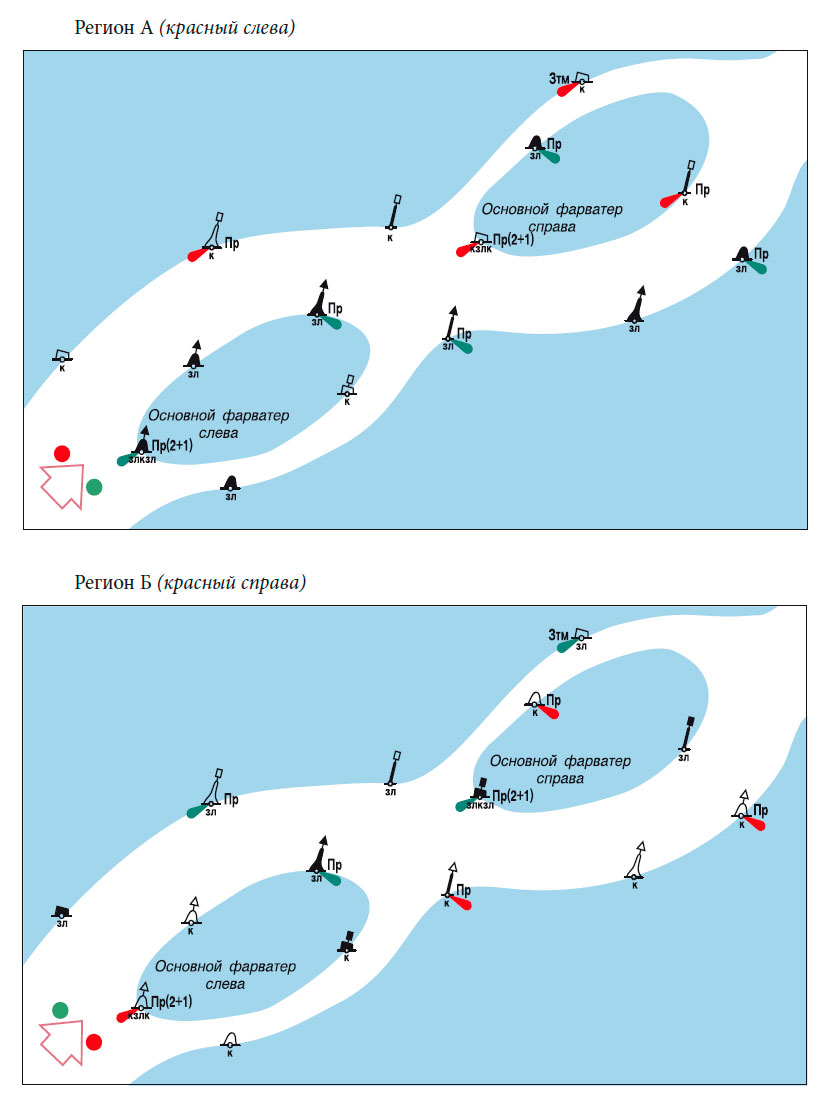
\includegraphics[width=0.8\linewidth]{mams_chart.jpeg}
  \caption{Обозначения на картах}
  \label{fig:mams-chart}
\end{figure*}

\begin{figure}[!htb]
  \centering{}
  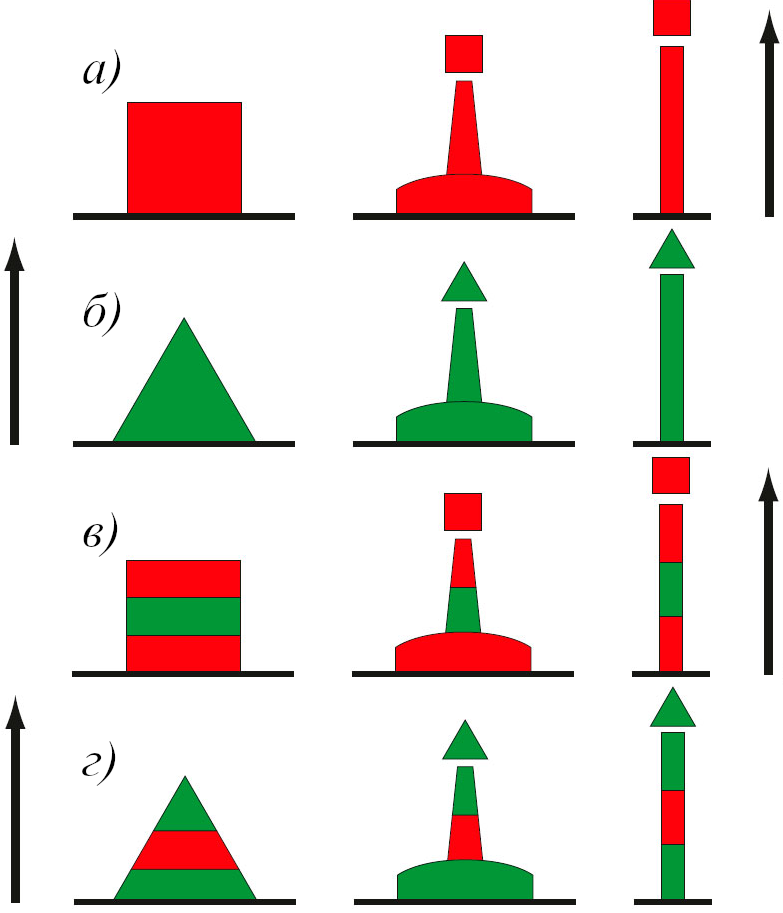
\includegraphics[width=0.8\linewidth]{mams_lateral_a.png}
  \caption{Латеральные знаки, регион А}
  {\small \textit{а} \--- знаки левой стороны;
    \textit{б} \--- знаки правой стороны;
    \textit{в} \--- основной фарватер справа;
    \textit{г} \--- основной фарватер слева}
  \label{fig:mams-lateral-a}
\end{figure}

\begin{figure}[!htb]
  \centering{}
  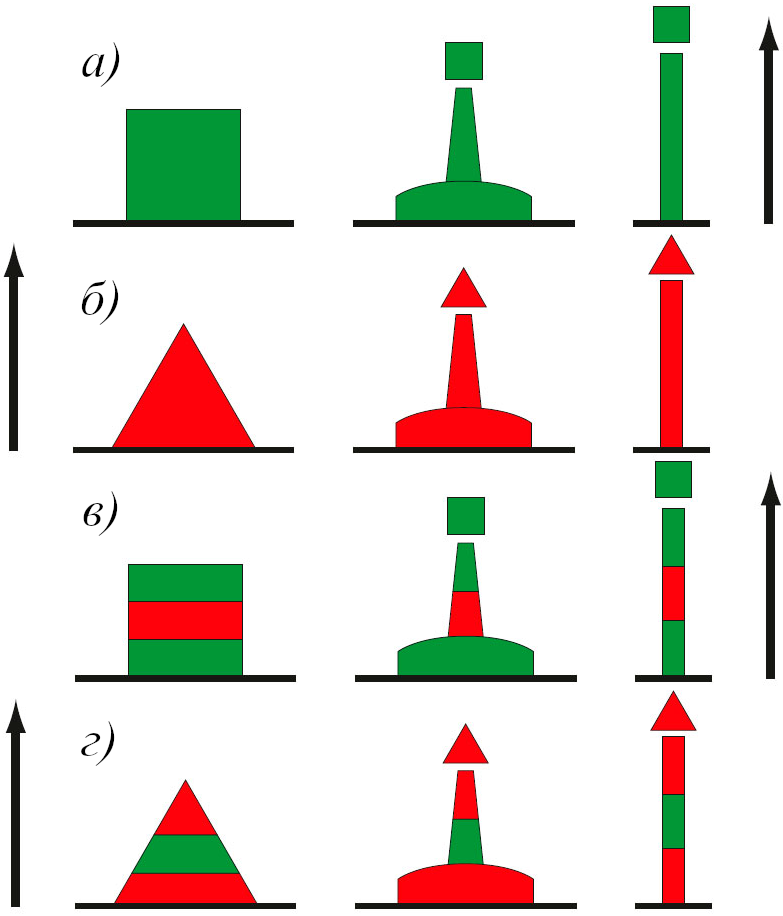
\includegraphics[width=0.8\linewidth]{mams_lateral_b.png}
  \caption{Латеральные знаки, регион Б}
  \label{fig:mams-lateral-b}
\end{figure}

\textbf{Латеральные знаки}\index{латеральная система} (знаки левой и
правой стороны), см.~\rris{mams-chart}, \rris{mams-lateral-a}
и~\rris{mams-lateral-b} \--- выставляются по принципу ограждения
сторон фарватера.  Стороны ограждаются буями или вехами. На корпусах
буев могут наноситься цифры или буквы. Нумерация буев по возрастающей
величине или обозначение буквами в алфавитной последовательности
ведётся со стороны моря.

В местах разделения фарватеров для обозначения основного
(предпочтительного) фарватера используются видоизменённые латеральные
знаки.

В регионе А на латеральных знаках, выставляемых на левой и правой
сторонах фарватера, зажигаются соответственно красные и зелёные огни.

В регионе Б на латеральных знаках, выставляемых на левой и правой
сторонах фарватера, зажигаются соответственно зелёные и красные огни.

\begin{figure}[!htb]
  \centering{}
  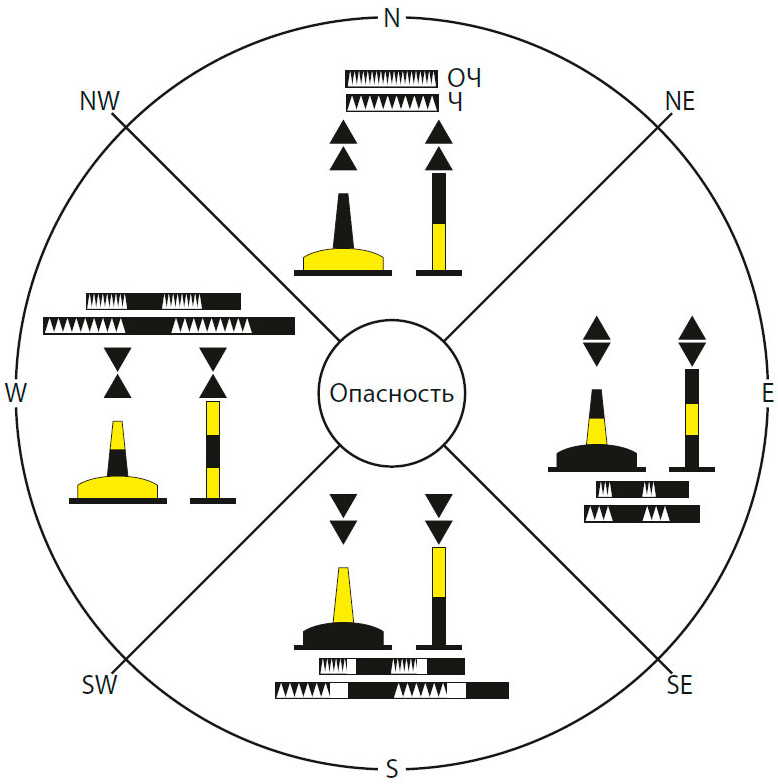
\includegraphics[width=0.8\linewidth]{mams_cardinal.png}
  \caption{Кардинальные знаки}
  \label{fig:mams-cardinal}
\end{figure}

\textbf{Кардинальные знаки}\index{кардинальная система},
см.~\rris{mams-cardinal}, выставляются по принципу ограждения
навигационных опасностей относительно стран света и обозначают
сторону, с какой следует обходить ограждаемую опасность. С этой целью
горизонт вокруг навигационной опасности условно делится на секторы:
северный $N$ \--- между румбами $NW$ и $NE$, восточный $E$ \--- между румбами
$NE$ и $SE$, южный $S$ \--- между румбами $SE$ и $SW$ и западный $W$ \--- между
румбами $SW$ и $NW$.

Кардинальные знаки выставляются в одном, нескольких или во всех
секторах и по их наименованию подразделяются на северные, восточные,
южные и западные. Буи и вехи выставляются: северные к $N$, восточные к
$E$, южные к $S$, западные к $W$ от опасности.  Для кардинальных знаков
определённая форма не установлена, но, как правило, они представляют
собой столбовидные буи и вехи.

Топовая фигура на кардинальных знаках имеет вид двух чёрных конусов.

Кардинальные знаки имеют особую систему проблесковых огней с
характером \--- очень частый ОЧ (100 или 120 проблесков в минуту) или
частый Ч (50 или 60 проблесков в минуту).

Цвет огня кардинальных знаков белый.

Число частых или очень частых проблесков 3; 6 или 9, установленное для
кардинальных знаков, избрано для облегчения их запоминания с учётом
того, что расположение знаков относительно опасности и число
проблесков ассоциируется с расположением соответствующих цифр на
циферблате часов.

Длительный проблеск продолжительностью не менее 2 с для огней южных
кардинальных знаков установлен с целью отличия их от огней, имеющих 3
или 9 очень частых или частых проблесков.

\begin{itemize}
\item Северный \--- ОЧ или Ч.
\item Восточный \--- ОЧ (3) или Ч (3) - три очень частых или частых
  проблеска с последующей темнотой.
\item Южный \--- ОЧ (6) ДлПр или Ч (6) ДлПр - шесть очень частых или
  частых проблесков с последующим длительным проблеском
  продолжительностью не менее 2 с, за которым следует темнота.
\item Западный \--- ОЧ (9) или Ч (9) - девять очень частых или частых
  проблесков с последующей темнотой.
\end{itemize}

\begin{figure}[!htb]
  \centering{}
  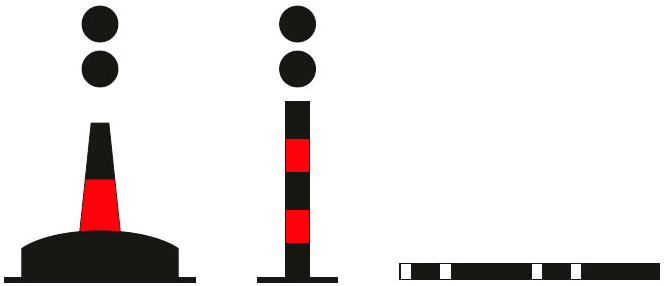
\includegraphics[width=0.8\linewidth]{mams_dangerous.png}
  \caption{Знаки ограждения отдельных опасностей}
  \label{fig:mams-dangerous}
\end{figure}

\textbf{Знаки, ограждающие отдельные опасности}\index{ограждение!отдельные опасности},
см.~\rris{mams-dangerous}, незначительных размеров, выставляются
непосредственно над опасностью и могут быть обойдены с любой
стороны. Знаки, ограждающие отдельные опасности, окрашены в чёрный
цвет с одной или несколькими красными горизонтальными полосами.

Топовая фигура имеет вид двух чёрных шаров, расположенных один над
другим. Характер огня \--- проблесковый (2 Пр), цвет огня \--- белый.

\begin{figure}[!htb]
  \centering{}
  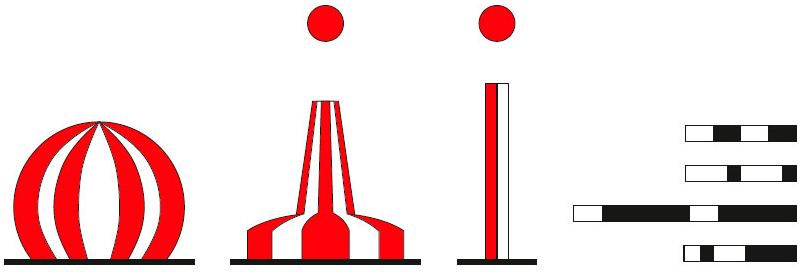
\includegraphics[width=0.8\linewidth]{mams_axial.png}
  \caption[Осевые знаки]{Осевые знаки или знаки чистой воды}
  \label{fig:mams-axial}
\end{figure}

\textbf{Осевые знаки}, или \textbf{знаки чистой воды},
\index{знаки!осевые}\index{знаки!чистой воды}
см.~\rris{mams-axial}, служат для обозначения оси фарватера или в
качестве подходных. Они представляют собой буи сферической или
столбовидной формы и вехи с топовой фигурой в виде красного шара. Эти
знаки являются единственным типом знаков, которые окрашены
вертикальными полосами (красными или белыми).  На знаках могут
зажигаться белые огни с характером:
\begin{itemize}
\item Изо - изофазный,
\item Зтм - затмевающийся,
\item ДлПр - длительно-проблесковый;
\item Мо (А) ($\cdot\ -$) — буква А по азбуке Морзе.
\end{itemize}

\begin{figure}[!htb]
  \centering{}
  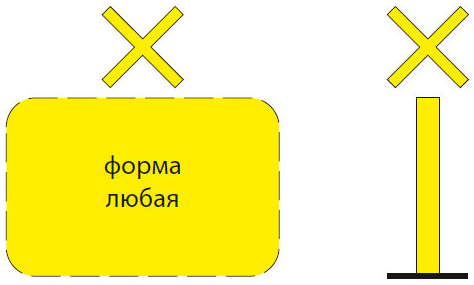
\includegraphics[width=0.8\linewidth]{mams_special.png}
  \caption{Знаки специального назначения}
  \label{fig:mams-special}
\end{figure}

\textbf{Знаки специального назначения}\index{знаки!специального назначения}, см.~\rris{mams-special},
предназначены для обозначения специальных районов или объектов,
показанных на картах или описанных в других навигационных документах,
например знаки, ограждающие районы свалки грунта, подводные кабели и
трубопроводы, обозначающие районы военных учений и зоны отдыха и
другие подобные районы.

Знаки специального назначения имеют жёлтую окраску. На знаках может
устанавливаться топовая фигура в виде жёлтого косого креста. Сами
знаки могут иметь любую форму. На знаках зажигаются жёлтые огни,
характеристика которых (Пр) отличается от характеристики белых огней
других знаков.  На корпусе буев специального назначения могут
наноситься цифры или буквы, позволяющие определить их назначение.

\textbf{Ограждение <<новых опасностей>>}\index{ограждение!новых опасностей}.
Термин <<новая опасность>> служит для обозначения опасностей,
ещё не описанных в навигационных документах.

При ограждении новых опасностей используется дублирование обычных
ограждающих знаков. Знак, ограждающий новую опасность, может быть
оборудован радиолокационным маяком-ответчиком с опознавательным
сигналом <<Д>> ($-\ \cdot\ \cdot$) по азбуке Морзе.

\onecolumn

%%% Local Variables:
%%% mode: latex
%%% TeX-master: "yacht-captain"
%%% End:
